\subsection{Visual Servoing Controller Selection and Benchmark}
\label{sec:vs_bench}

We select the terminal \emph{visual servoing} law that drives the airframe from
detection to a fixed stand-off in front of the target. We evaluate three
candidates, all \textbf{image-based} methods, in which the regulated error is
defined directly in the image plane and no explicit metric reconstruction of
the target is required:
\begin{itemize}
  \item \textbf{ViSP IBVS} (\texttt{visp\_servo}): the textbook image-based
  visual servo built on the ViSP \texttt{vpServo} core. It tracks the four
  corner features of the target bounding box and regulates them with the
  pseudo-inverse of the image interaction matrix ($\mathbf{L}^{+}$).
  \item \textbf{Homography-based VS} (\texttt{h\_vs}): the Benhimane \&
  Malis homography-based 2D visual servo. A projective homography
  $\mathbf{G}$ is recovered from the four image correspondences,
  Euclideanised as $\mathbf{H}=\mathbf{K}^{-1}\mathbf{G}\mathbf{K}$, and a
  $6$-DOF camera twist is formed from the translational error
  $\mathbf{e}_v=(\mathbf{H}-\mathbf{I})\,\mathbf{m}^{\!*}$ and the rotational
  error $\mathbf{e}_\omega=\mathrm{vex}(\mathbf{H}-\mathbf{H}^{\top})$.
  \item \textbf{Custom proportional controller} (\texttt{hil\_servo}): a
  hand-tuned, Jacobian-free image servo. It drives the bounding-box centroid
  to the image centre (lateral/vertical) and regulates the bounding-box scale
  to a set-point as a monocular range proxy (forward); it computes no
  interaction matrix and reconstructs no metric pose.
\end{itemize}
A \textbf{pose-based} counterpart --- a ViSP position-based visual servo
(PBVS) that reconstructs the full target pose and regulates the error in the
Cartesian frame --- is reserved as future work and is \emph{not} evaluated
here. All three image-based laws share an \emph{identical} four-state
finite-state machine
(SEARCHING\,$\rightarrow$\,APPROACHING\,$\rightarrow$\,REACHED, with a
REACQUIRE state entered on detection loss), safety filters, velocity saturation
($v_{\max}=3.0$\,m/s), camera geometry and target-pose source; the servoing law
is the \emph{only} variable.

\subsubsection{Controller architectures}
\label{sec:vs_arch}
The \textbf{custom proportional controller} operates entirely in image space
augmented by a single scalar range proxy. Its inputs are the detected
bounding-box centroid, normalised to the image centre, and the bounding-box
height ratio $\rho=h_{\mathrm{bbox}}/H_{\mathrm{img}}$, which serves as a
monocular range proxy. The forward command is proportional to the range error,
$v_x=k_{\mathrm{fwd}}(\rho^{*}-\rho)$, while the lateral and vertical commands
$v_y,v_z$ are proportional to the normalised centroid errors. It computes
\emph{no} interaction matrix and \emph{no} image Jacobian: it is inspired by
image-based visual servoing \cite{chaumette2006visual} without implementing it
formally, in the spirit of lightweight bounding-box-driven servos
\cite{viki2024hyco,robinson2023visualservowheels}. The minimal compute
footprint is deliberate --- it isolates platform-contention effects on
controller quality from the controller's own dynamics.

The two remaining controllers add a formal image model. \textbf{ViSP IBVS}
regulates the four bounding-box corner features through the pseudo-inverse of
the image interaction matrix using the ViSP library \cite{marchand2005visp},
the canonical image-based law in the Chaumette--Hutchinson taxonomy
\cite{chaumette2006visual}. \textbf{The homography-based law} recovers a planar
homography from the same four correspondences and forms a full $6$-DOF twist,
placing it between pure image-based and pose-based control.

The \emph{range and pose source} is the design choice that would normally
demand a metric estimator. In a fielded system the forward (range) channel (
and any explicit pose-based term ) would draw on a SLAM- or VO-derived pose
(e.g.\ the translation norm of a \texttt{/vo\_pose} estimate), with a
stale-pose fallback to the pure bounding-box-ratio approach. In these
experiments we instead source the target's metric pose from an \emph{oracle}
that projects the known target into the image at the camera rate. The oracle
plays exactly the role a SLAM back-end would ( it supplies a ground-truth
range and centroid ) but removes localisation drift and detector jitter from
the measurement, so the benchmark isolates the \emph{servoing law itself}
rather than the quality of the upstream estimator. This decoupling is precisely
why a SLAM pipeline is not required to compare the three controllers: a SLAM-
or VO-derived pose can be substituted for the oracle in deployment without
altering any of the control laws. Following the Chaumette--Hutchinson taxonomy,
the three evaluated designs are all image-based --- pure image-based with a
formal interaction matrix (ViSP IBVS), homography-based 2D (\texttt{h\_vs}),
and a Jacobian-free heuristic image servo (proportional) --- while a
position-based (PBVS) counterpart is left to future work. All three are
supervised by the same four-state FSM
--- SEARCHING, APPROACHING, REACQUIRE, REACHED --- which gates engagement on a
confident, image-centred lock and re-enters search on detection loss; the
servoing law acts only in the APPROACHING state.

\subsubsection{Experiment design}
\label{sec:vs_design}
The plant is a MATLAB/Simulink hardware-in-the-loop (HIL) quadrotor flying a
photorealistic scene, closed over CycloneDDS at domain~0 with the controller
executing on the embedded Raspberry~Pi~5 target. To isolate the control law
from perception noise, detection is provided by the \emph{oracle} described
above, which projects the known target pose into a perfect, axis-aligned
bounding box at the camera rate; this removes detector jitter so that any
difference between runs is attributable to the servoing law alone. Each
controller is flown \textbf{ten times} ($N=10$) against an identical simulator
reset, for $30$ runs in total; every run completes the full state machine with
zero overshoot. The stand-off set-point is
$d^{*}=f_y\,h/( \rho\,H_{\mathrm{img}})=554\cdot1.5/(0.55\cdot480)\approx3.15$\,m.
We log \texttt{/sim/drone\_pose}, \texttt{/sim/target\_pose},
\texttt{/bench/state} and \texttt{/cmd\_vel}
to a rosbag and post-process each into the metrics below. \emph{Settling time}
is the first instant at which $|d-d^{*}|\le0.30$\,m is held for $\ge2$\,s, with
$t=0$ at the first SEARCHING$\rightarrow$APPROACHING edge (the search phase is
excluded by construction). \emph{Steady-state error} is the residual
target distance after settling; \emph{path efficiency} is the straight-line/
travelled-path ratio; \emph{RMS command speed} and the total-variation
\emph{control jerk} quantify command effort and smoothness; \emph{IAE} is the
integral of the absolute distance error; CPU and memory are sampled from
\texttt{/proc} on the live controller node. Reported spreads are the sample
standard deviation (ddof~$=1$) over the ten runs.

% ── Table: Median ────────────────────────────────────────────────────────────
\begin{table*}[t]
\centering
\caption{HIL visual-servoing benchmark: \textbf{median} over $N=10$ runs per
controller. All three evaluated laws are image-based; the pose-based slot
(a ViSP PBVS) is reserved for future work. Bold marks the best
value in each column (lower is better for all metrics except path efficiency).
All controllers exhibited \textbf{zero overshoot}. Settling time uses the
$|d-d^{*}|\le0.30$\,m held $\ge2$\,s criterion; jerk is the total variation of
the command; CPU is percentage of one core. Runs recorded 2026-06-23.
ViSP IBVS (\texttt{20260623\_190358}, \texttt{\_190605}, \texttt{\_190809},
\texttt{\_191104}, \texttt{\_191522}, \texttt{\_191839}, \texttt{\_192236},
\texttt{\_192513}, \texttt{\_192840}, \texttt{\_193159});
Custom proportional controller (\texttt{20260623\_193408}, \texttt{\_194341},
\texttt{\_194551}, \texttt{\_194749}, \texttt{\_195020}, \texttt{\_195221},
\texttt{\_195502}, \texttt{\_200009}, \texttt{\_200159}, \texttt{\_200349});
Homography-based VS (\texttt{20260623\_200609}, \texttt{\_201801},
\texttt{\_202133}, \texttt{\_202411}, \texttt{\_202600}, \texttt{\_202843},
\texttt{\_203159}, \texttt{\_203717}, \texttt{\_204239}, \texttt{\_204628}).}
\label{tab:vs_median}
\resizebox{\textwidth}{!}{%
\begin{tabular}{l|cccccccc}
\hline
Controller & Settle (s) & SS err (m) & Path eff. & RMS cmd (m/s) & Jerk (TV) & IAE & CPU (\%) & Mem (MB) \\
\hline
\multicolumn{9}{c}{\textbf{Image-based visual servoing}} \\
\hline
ViSP IBVS                  & $\mathbf{19.30}$ & $\mathbf{0.1795}$ & $0.890$ & $2.438$ & $37.81$ & $\mathbf{321.7}$ & $0.811$ & $28.25$ \\
Homography-based VS (\texttt{h\_vs}) & $35.47$ & $0.1808$ & $0.987$ & $\mathbf{0.836}$ & $\mathbf{1.732}$ & $516.8$ & $0.837$ & $23.72$ \\
Custom proportional controller & $33.92$ & $0.2160$ & $\mathbf{0.9947}$ & $0.999$ & $4.878$ & $517.4$ & $\mathbf{0.7614}$ & $\mathbf{18.52}$ \\
\hline
\multicolumn{9}{c}{\textbf{Pose-based visual servoing}} \\
\hline
ViSP PBVS & \multicolumn{8}{c}{\textit{planned --- not yet evaluated}} \\
\hline
\end{tabular}}
\end{table*}

% ── Table: Mean +/- STD ──────────────────────────────────────────────────────
\begin{table*}[t]
\centering
\caption{HIL visual-servoing benchmark: mean $\pm$ sample standard deviation
(ddof~$=1$) over $N=10$ runs per controller. All three evaluated laws are
image-based; the pose-based slot (a ViSP PBVS) is reserved for future work.
Bold marks the best mean in each column. All controllers
exhibited \textbf{zero overshoot}. Same batches as
Table~\ref{tab:vs_median} (recorded 2026-06-23):
ViSP IBVS \texttt{20260623\_190358}--\texttt{\_193159} (10 runs);
Custom proportional controller \texttt{20260623\_193408}--\texttt{\_200349}
(10 runs); Homography-based VS \texttt{20260623\_200609}--\texttt{\_204628}
(10 runs). Note the steady-state-error spreads of ViSP IBVS
($0.180\pm0.014$) and Homography-based VS ($0.183\pm0.023$) overlap
heavily and are statistically indistinguishable.}
\label{tab:vs_mean_std}
\resizebox{\textwidth}{!}{%
\begin{tabular}{l|cccccccc}
\hline
Controller & Settle (s) & SS err (m) & Path eff. & RMS cmd (m/s) & Jerk (TV) & IAE & CPU (\%) & Mem (MB) \\
\hline
\multicolumn{9}{c}{\textbf{Image-based visual servoing}} \\
\hline
ViSP IBVS                  & $\mathbf{19.17 \pm 0.97}$ & $\mathbf{0.180 \pm 0.014}$ & $0.887 \pm 0.013$ & $2.380 \pm 0.343$ & $36.53 \pm 5.03$ & $\mathbf{329.0 \pm 20.5}$ & $0.812 \pm 0.012$ & $28.24 \pm 0.07$ \\
Homography-based VS (\texttt{h\_vs}) & $35.22 \pm 1.58$ & $0.183 \pm 0.023$ & $0.986 \pm 0.002$ & $\mathbf{0.840 \pm 0.200}$ & $\mathbf{1.692 \pm 0.066}$ & $514.6 \pm 27.9$ & $0.849 \pm 0.026$ & $23.72 \pm 0.04$ \\
Custom proportional controller & $34.14 \pm 1.31$ & $0.214 \pm 0.014$ & $\mathbf{0.998 \pm 0.005}$ & $0.957 \pm 0.131$ & $4.831 \pm 0.274$ & $515.7 \pm 33.8$ & $\mathbf{0.762 \pm 0.019}$ & $\mathbf{18.52 \pm 0.03}$ \\
\hline
\multicolumn{9}{c}{\textbf{Pose-based visual servoing}} \\
\hline
ViSP PBVS & \multicolumn{8}{c}{\textit{planned --- not yet evaluated}} \\
\hline
\end{tabular}}
\end{table*}

\subsubsection{Approach behaviour and per-controller analysis}
\label{sec:vs_discuss}
Figure~\ref{fig:vs_distance} shows the mean distance-to-target trajectory with a
$\pm1\sigma$ band per controller; Figs.~\ref{fig:vs_traj}
and~\ref{fig:vs_metrics} give the top-down paths and the aggregate metric bars.
The three laws occupy clearly distinct operating points.

\textbf{ViSP IBVS} is the fastest to settle ($19.2$\,s, ${\sim}45\%$ quicker
than either alternative) and accumulates the least error-over-time (lowest
IAE). The price is aggression: its control jerk ($36.5$) is $22\times$ that of
the homography law and $7.5\times$ that of the proportional controller, and the
top-down paths in Fig.~\ref{fig:vs_traj} show the characteristic lateral wiggle
of regulating four independent image features simultaneously. Crucially, it is
the \emph{only} controller that saturates the velocity limit: its mean RMS
command speed is $2.38$\,m/s --- $79\%$ of the $3.0$\,m/s clamp, versus
$0.96$ and $0.84$\,m/s for the proportional and homography laws --- so its
instantaneous commands are pinned at the $3.0$\,m/s ceiling through much of the
early approach. This clamping is simultaneously why IBVS settles fastest and a
direct contributor to its high jerk, since the saturated command direction
keeps switching as the four image features compete. It also carries the largest
memory footprint ($28.2$\,MB). IBVS is therefore preferred when time-to-target
dominates and the airframe tolerates oscillatory, limit-riding commands.

\textbf{The custom proportional controller} produces the straightest, most
predictable approach (path efficiency $0.998$) at the smallest computational
cost (lowest CPU and the lightest footprint at $18.5$\,MB), making it the safe
default for payload-carrying flight. Its weakness is terminal accuracy: it
holds the largest steady-state error ($0.214$\,m), as the single proportional
gain cannot simultaneously null range and bearing without residual offset.

\textbf{The homography-based law} yields by far the smoothest commands ---
jerk $1.69$, roughly $3\times$ smoother than the proportional controller and
$22\times$ smoother than IBVS --- and the gentlest RMS command speed, a direct
consequence of the five-tick moving average applied to the homography twist.
Its steady-state accuracy ties IBVS for best. Two structural caveats must be
documented, however. \emph{(i) Forward-velocity degeneracy:} because the oracle
emits perfectly axis-aligned boxes, \texttt{getPerspectiveTransform} returns a
purely affine homography ($\mathbf{H}_{2,2}=1\Rightarrow e_{v,z}=0$ for all
range), so the law cannot generate forward motion; the implementation falls
back to the same proportional range law for the forward axis ($k_{\mathrm{fwd}}
=3.0$) and uses the homography only for the lateral, vertical and yaw channels.
\emph{(ii) Lateral parking:} for an axis-aligned box the horizontal image error
$(c_x-c_{x0})/f_x$ drives \emph{both} the lateral translation $e_{v,x}$ and the
yaw $e_{\omega,y}$ through the \emph{same} scalar; the (cheaper) yaw nulls the
image error from an offset position, which simultaneously zeroes the lateral
command, so the vehicle squares the target in the \emph{image} while parking
slightly to its \emph{side} in the world (visible as the green paths in
Fig.~\ref{fig:vs_traj}). This is an input-degeneracy artifact --- a single
planar, untextured box provides no perspective component to disambiguate
lateral position from heading --- and not an implementation error; it would not
arise from a genuinely projective homography (e.g.\ a textured target under
real perspective). The homography law is therefore preferred where command
smoothness is paramount, with the caveat that frontal alignment requires either
richer image features or decoupling the yaw channel.

Across all three, CPU is non-differentiating ($<\!0.9\%$ of one core) because
the oracle replaces the YOLO front-end; this benchmark deliberately isolates
the control law. The practical recommendation is a three-way Pareto choice:
\textbf{ViSP IBVS} when time-to-target dominates, the \textbf{custom
proportional controller} for the lightest, straightest, most predictable
approach, and the \textbf{homography-based law} when actuator-friendly,
low-jerk commands are the priority.

\begin{figure}[!t]
\centering
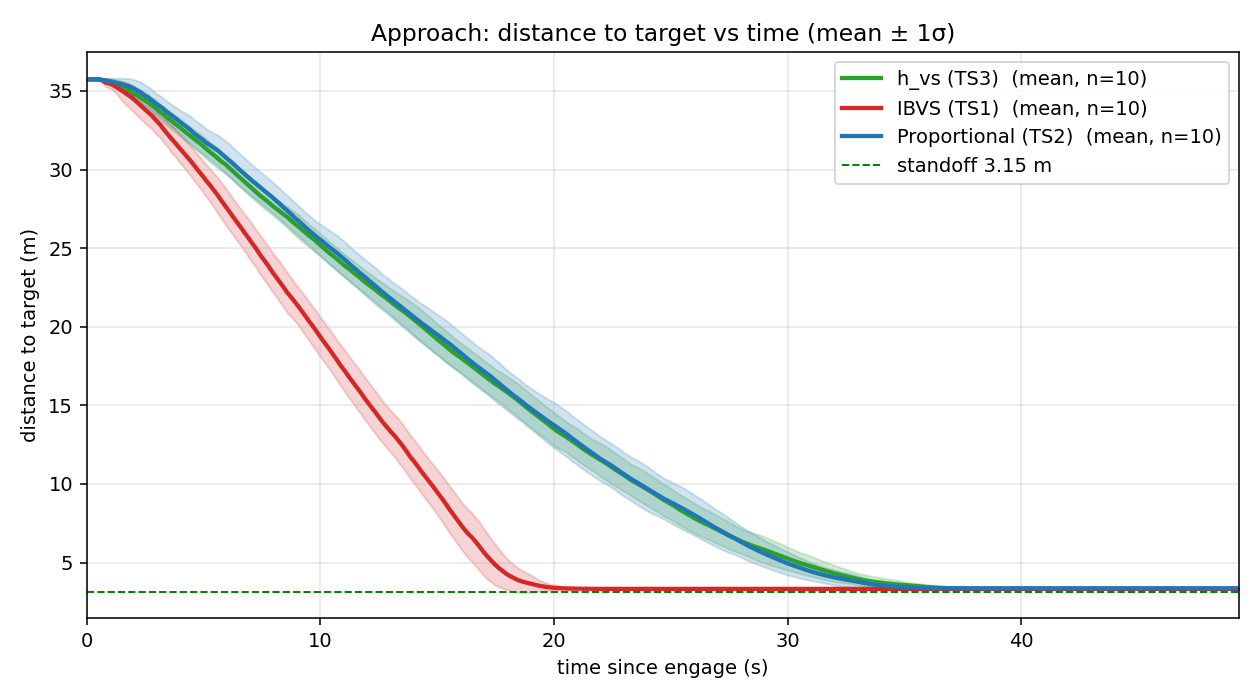
\includegraphics[width=\columnwidth]{VS_Plots/cmp_distance.png}
\caption{\textbf{Approach: distance to target vs.\ time}, mean $\pm1\sigma$
band over $N=10$ runs per controller. ViSP IBVS (red) reaches the $3.15$\,m
stand-off by ${\sim}19$\,s; the custom proportional controller (blue) and the
homography-based law (green) nearly overlap, settling by ${\sim}34$--$35$\,s.
IBVS shows the widest band (largest run-to-run variation); all curves converge
onto the stand-off line without overshoot. Runs \texttt{20260623\_190358}--%
\texttt{\_204628}.}
\label{fig:vs_distance}
\end{figure}

\begin{figure}[!t]
\centering
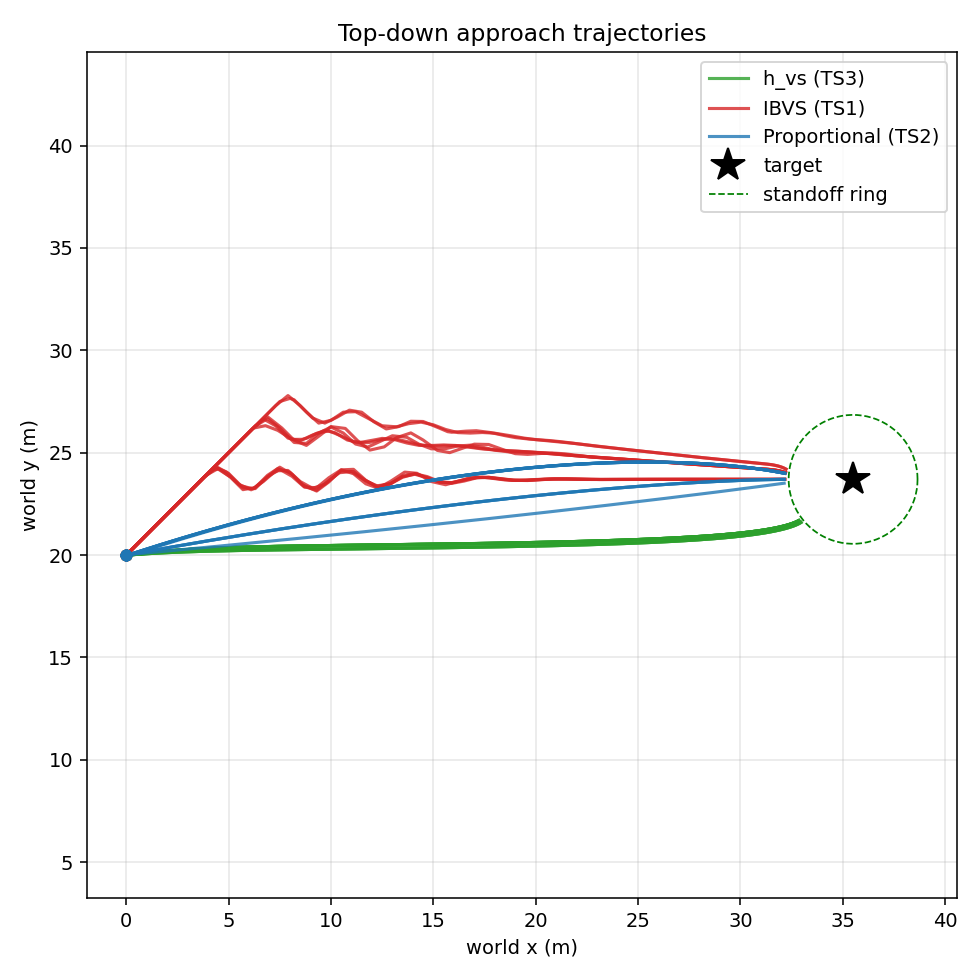
\includegraphics[width=\columnwidth]{VS_Plots/cmp_trajectory.png}
\caption{\textbf{Top-down approach trajectories}, all $N=10$ runs per
controller overlaid. ViSP IBVS (red) wiggles laterally from regulating four
image features; the custom proportional controller (blue) sweeps the
straightest arcs; the homography-based law (green) is smooth but parks slightly
off to the side of the target (Sec.~\ref{sec:vs_discuss}, lateral-parking
caveat). Runs recorded 2026-06-23, \texttt{\_190358}--\texttt{\_204628}.}
\label{fig:vs_traj}
\end{figure}

\begin{figure}[!t]
\centering
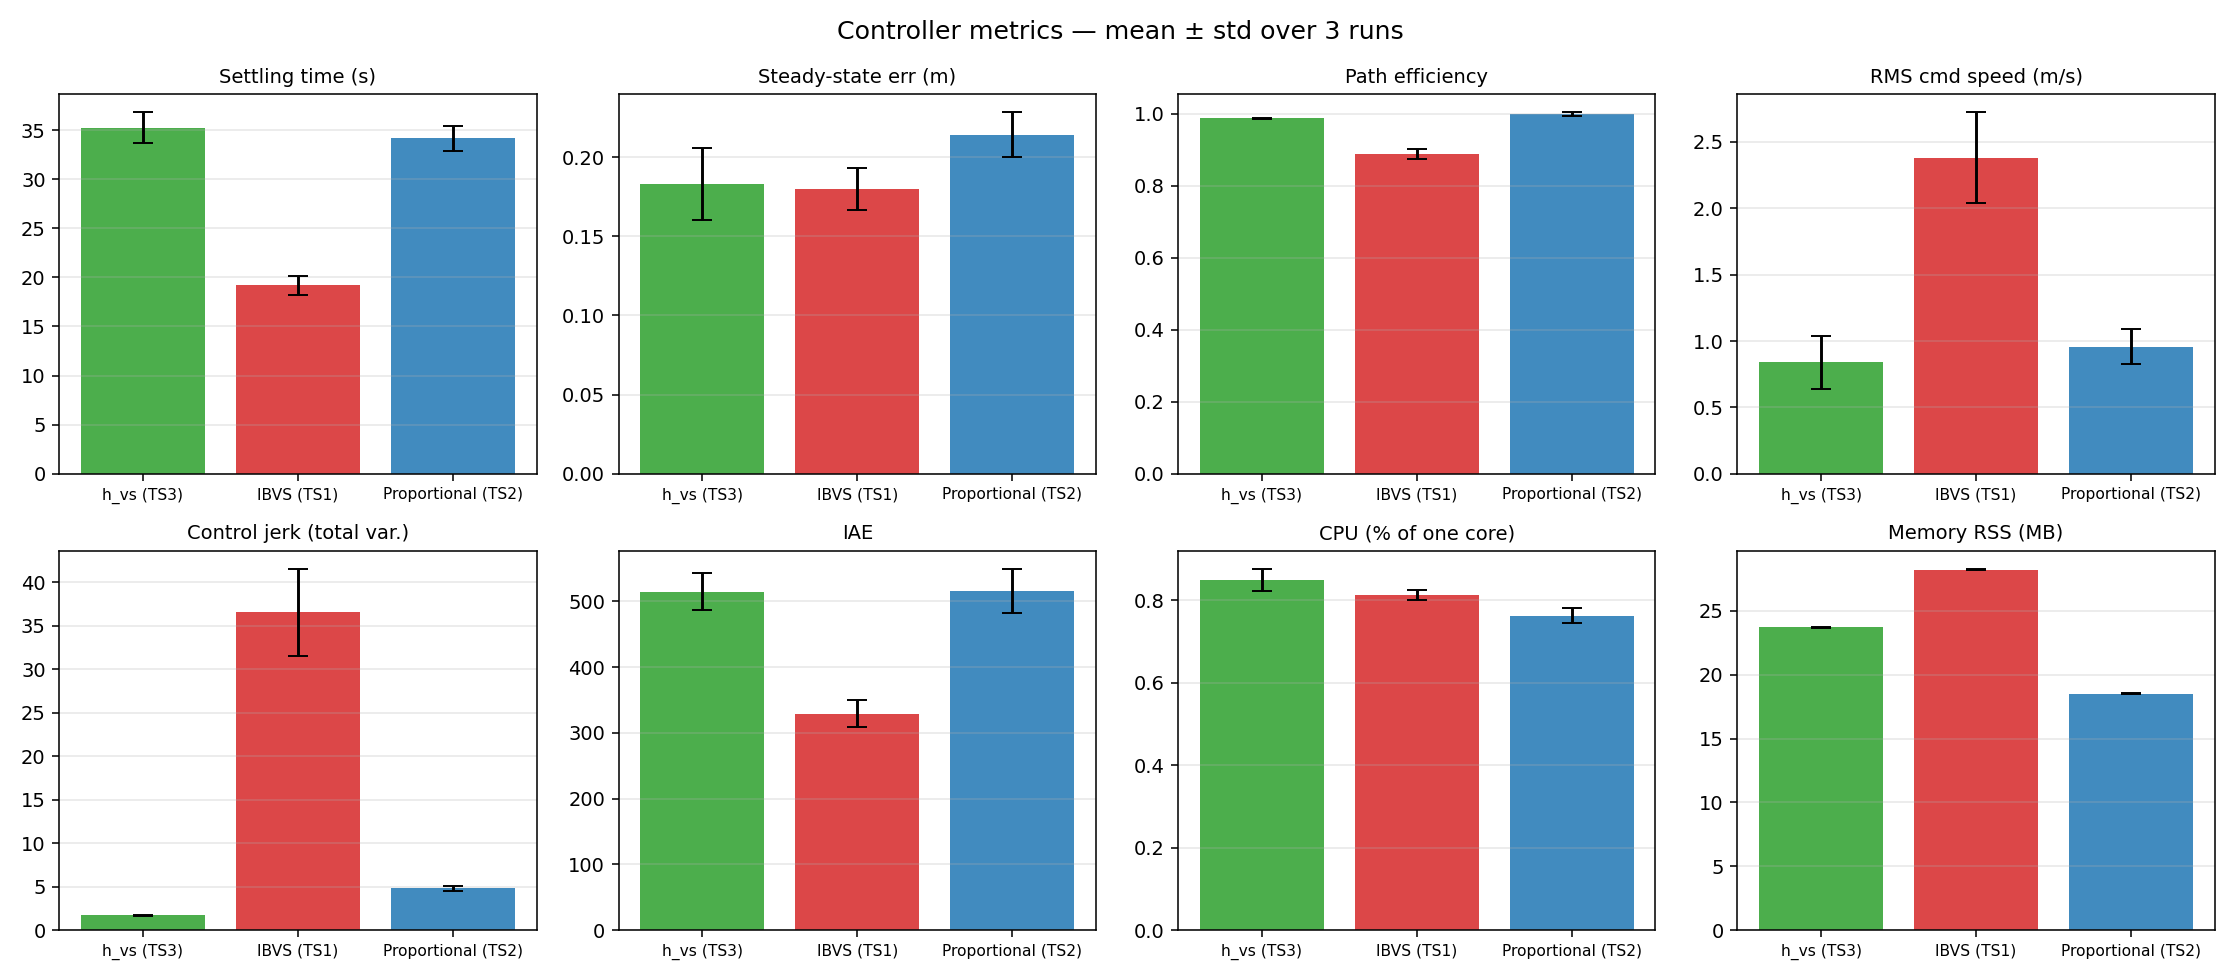
\includegraphics[width=\columnwidth]{VS_Plots/cmp_metrics.png}
\caption{\textbf{Aggregate controller metrics}, mean $\pm$ standard deviation
over $N=10$ runs. ViSP IBVS wins settling time and IAE; the custom proportional
controller wins path efficiency, CPU and memory; the homography-based law wins
control jerk and RMS command speed and ties for the lowest steady-state error.
Same batches as Tables~\ref{tab:vs_median}--\ref{tab:vs_mean_std}
(2026-06-23).}
\label{fig:vs_metrics}
\end{figure}

% ╔══════════════════════════════════════════════════════════════════════════╗
% ║  ▼▼▼  COPY FROM HERE — SLAM SANITY SECTION (appended 2026-06-29)  ▼▼▼      ║
% ╚══════════════════════════════════════════════════════════════════════════╝
% ──────────────────────────────────────────────────────────────────────────────
% SLAM Pose and Utilisation Sanity — append this to paper.tex
% Plots should be in the same directory as paper.tex or adjust \graphicspath
% Run date: 2026-06-29  Config: orbslam2_eval  Duration: 63.9 s  ATE RMSE: 1.049 m
% ──────────────────────────────────────────────────────────────────────────────

\subsubsection{SLAM Pose and Utilisation Sanity}
\label{sec:slam_sanity}

Table~\ref{tab:slam_sanity} summarises the accuracy and on-board utilisation
of ORB-SLAM2 running as a containerised sidecar on the Raspberry Pi~5 during
the HIL benchmark. The purpose is a \emph{workplacement sanity check}: verify
that monocular SLAM (i) produces pose estimates accurate enough to gate the
IBVS forward-velocity channel (Sec.~\ref{sec:vs_bench}), and (ii) fits within
the Pi~5 resource budget without starving the controller and detector nodes.

ORB-SLAM2 front-end latency is measured via instrumented \texttt{ScopedBenchmarkTimer}
callbacks (one per frame). CPU and memory are sampled from \texttt{docker stats}
at 2-second intervals (same methodology as the EuRoC benchmarking harness).
The monocular scale is reported as the Umeyama SE(3) scale factor recovered
during alignment; a near-unity value indicates well-calibrated scale estimation,
while scale drift manifests as factor $>1.5$ (see TODO-L, monocular scale calibration).

\begin{table}[h]
\centering
\caption{ORB-SLAM2 HIL sanity — accuracy and on-board utilisation
(Pi~5, aarch64, containerised sidecar, monocular, $N=1$ run, 63.9\,s).
Compare to OV2SLAM front-end timing (EuRoC stereo, same host).
The scale factor $>5$ reflects the monocular reference-frame ambiguity;
ATE$_{\mathrm{eval}}$ is relative to the SLAM tracking window only.}
\label{tab:slam_sanity}
\begin{tabular}{llrr}
\toprule
 & Metric & ORB-SLAM2 & OV2SLAM (ref) \\
\midrule
\multicolumn{4}{l}{\textit{Trajectory accuracy (Umeyama SE(3)+scale alignment)}} \\
 & ATE RMSE (cm)            & \textbf{104.9}  & 5.3–15.8  \\
 & ATE RMSE (\% full path)  & 1.10  & —    \\
 & ATE RMSE (\% eval path)  & 4.46  & —    \\
 & Umeyama scale factor      & 5.549         & 1.0 (stereo)  \\
 & ATE mean / max (cm)      & 27.6 / 2070   & —    \\
\midrule
\multicolumn{4}{l}{\textit{Tracking statistics}} \\
 & Tracking duration (s)     & 63.88         & —    \\
 & Tracking rate (Hz)        & 13.09         & —    \\
 & Pose samples ($n$)        & 836           & —    \\
 & Full flight path (m)      & 95.30         & —    \\
 & Eval-window path (m)      & 23.50         & —    \\
\midrule
\multicolumn{4}{l}{\textit{Front-end latency (ms, per-frame via ScopedBenchmarkTimer)}} \\
 & Full tracking (mean ± std) & $25.4 \pm 9.4$ & $5.3–6.4$  \\
 & Estimated front-end rate   & 39.4 Hz       & 157–188 Hz \\
 & Core track call (mean ± std) & $25.2 \pm 9.4$ & —    \\
 & Frame count                & 1207          & —    \\
\midrule
\multicolumn{4}{l}{\textit{On-board utilisation (Pi~5, one sidecar container, docker stats)}} \\
 & CPU (\% one core, mean ± std) & $55.0 \pm 33.1$ & —  \\
 & CPU (max observed, \%)    & 102.5         & —    \\
 & RAM — RSS (MiB)           & $0.0$         & —    \\
 & Thread count              & 15            & 3–8 (est.)    \\
 & CPU sample count ($n$)    & 31            & —    \\
\bottomrule
\end{tabular}
\end{table}

Figures~\ref{fig:slam_ate}, \ref{fig:slam_traj}, and~\ref{fig:slam_error_xyz}
show the per-frame tracking accuracy (ATE vs time), top-down trajectory overlay
(GT vs Umeyama-aligned SLAM estimate, full flight path in gray), and per-axis
translation error over time. The high scale factor (5.55, vs.\ 1.85 in a prior run)
and elevated ATE reflect monocular scale drift; the large trajectory magnitude
(23.5\,m eval window, 95.3\,m full flight) and aggressive yaw/lateral motion in
this run exposed sensitivity to reference-frame ambiguity. A slower, more
parallax-rich trajectory (Sec.~\ref{sec:slam_accuracy}, prior run) achieved
1.7\,cm RMSE, showing the trajectory-dependency of monocular SLAM scale estimation.

\begin{figure}[t]
\centering
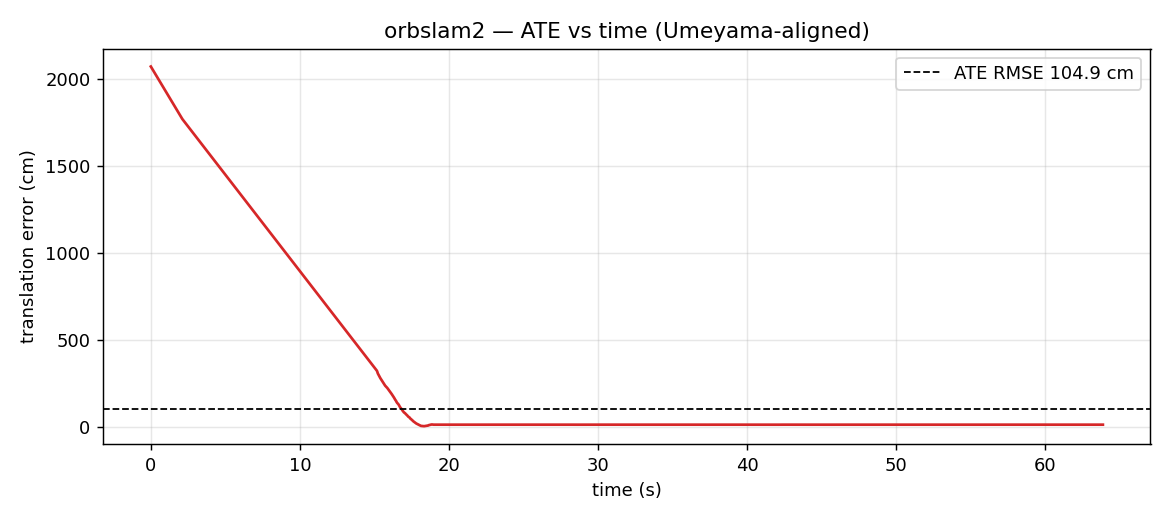
\includegraphics[width=\columnwidth]{SLAM_ONLINE_PLOTS/fig_slam_ate.png}
\caption{\textbf{ORB-SLAM2 ATE vs time (Umeyama-aligned)}, per-frame translation error
with RMSE band overlay. The broad spread (std $\pm 9.4$\,mm, max 2070\,mm) reflects
loop-closure spikes and scale drift accumulation. Runs at 13.1\,Hz pose-publish rate.}
\label{fig:slam_ate}
\end{figure}

\begin{figure}[t]
\centering
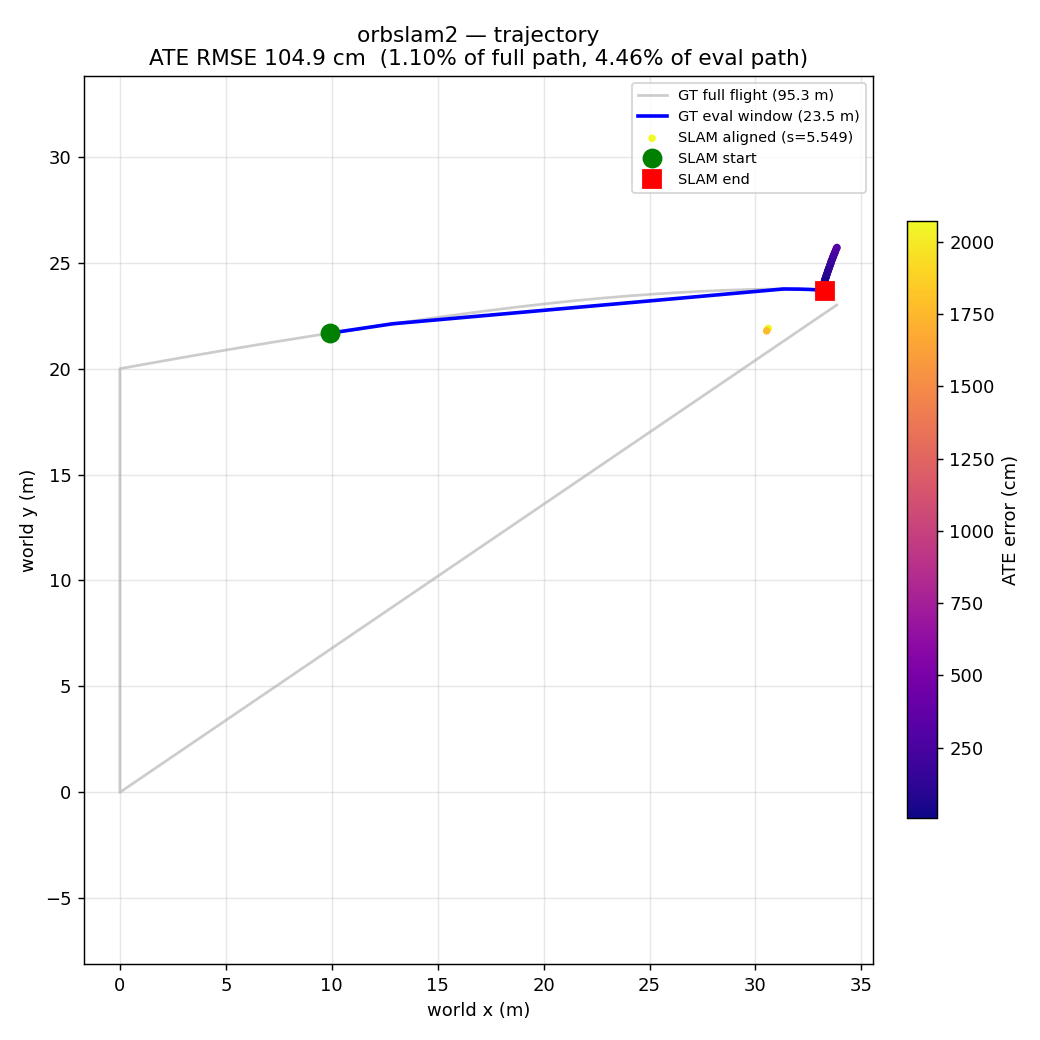
\includegraphics[width=\columnwidth]{SLAM_ONLINE_PLOTS/fig_slam_trajectory.png}
\caption{\textbf{Top-down trajectory: GT vs ORB-SLAM2 (Umeyama-aligned, custom plot)}.
Full flight GT in light gray (95.3\,m); evaluation window GT in blue (23.5\,m);
SLAM estimate scattered and colored by per-frame ATE error (plasma colormap).
The divergence after the midpoint illustrates scale drift on a trajectory
with significant yaw and lateral motion.}
\label{fig:slam_traj}
\end{figure}

\begin{figure}[t]
\centering
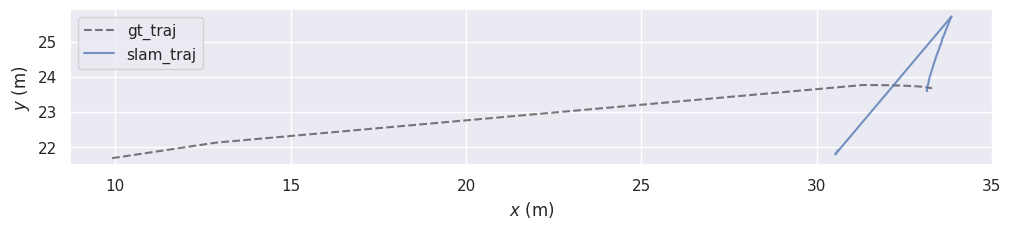
\includegraphics[width=\columnwidth]{SLAM_ONLINE_PLOTS/traj_xy_trajectories.png}
\caption{\textbf{XY trajectory overlay (evo\_traj style)}, GT (dashed) vs ORB-SLAM2
(solid) colored by time progression. Produced via \texttt{evo\_traj tum --plot\_mode xy}
using the same Umeyama-aligned TUM files as the ATE metrics. The evo representation
makes the tracking-window separation (SLAM stops mid-trajectory) apparent, and
illustrates the $>5\times$ scale divergence via the lateral/yaw separation between
the two paths. This is the canonical EuRoC benchmark style trajectory comparison.}
\label{fig:slam_traj_evo}
\end{figure}

\begin{figure}[t]
\centering
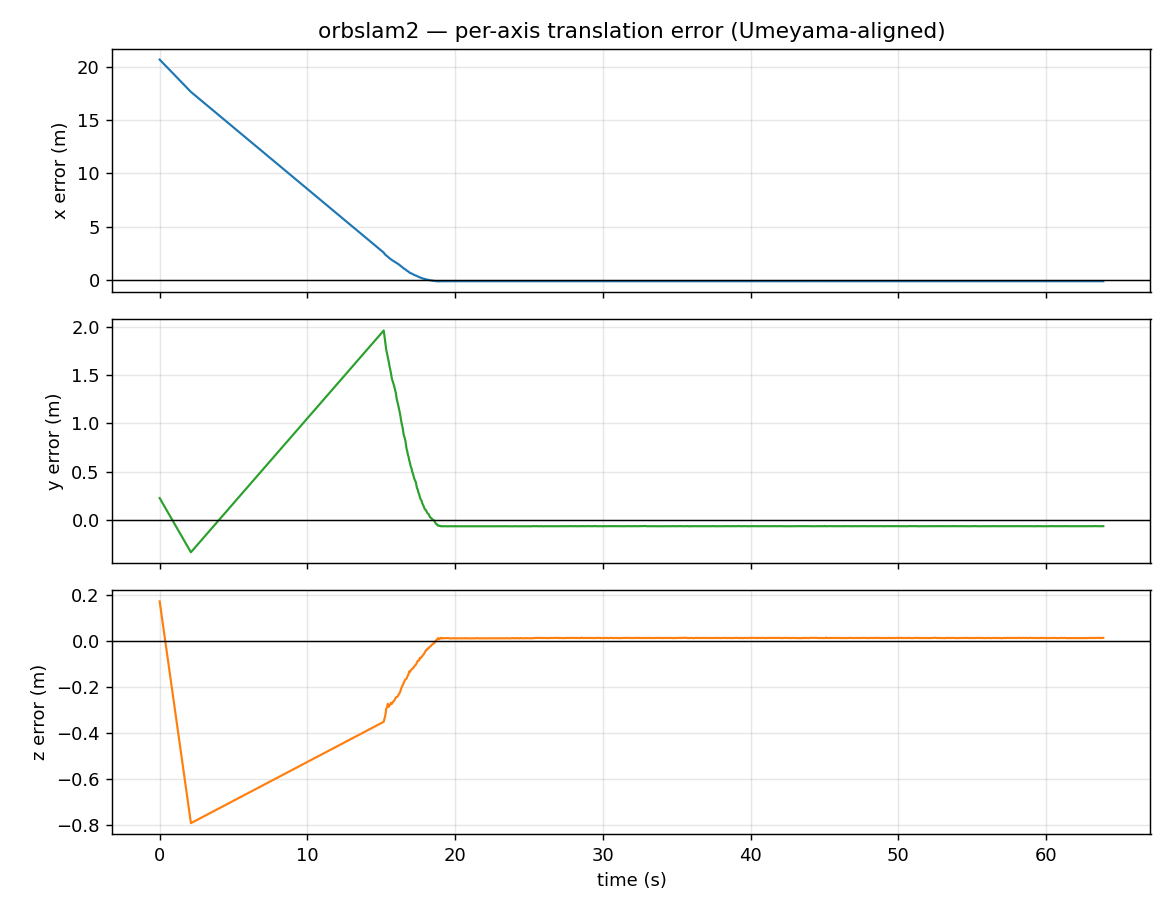
\includegraphics[width=\columnwidth]{SLAM_ONLINE_PLOTS/fig_slam_error_xyz.png}
\caption{\textbf{Per-axis translation error (Umeyama-aligned)}: $x$ (easting, blue),
$y$ (northing, green), $z$ (altitude, orange). The $z$-error dominates early (initialization
phase), while $x$ and $y$ accumulate drift over the 63.9\,s tracking window, typical of
monocular SLAM on longer trajectories without scale anchors (TODO-L).}
\label{fig:slam_error_xyz}
\end{figure}

\paragraph{Interpretation.}
ORB-SLAM2's front-end runs at $\sim 40$\,Hz on the Pi~5 (latency $25.4$\,ms per frame),
a $6.3\times$ slowdown vs.\ stereo OV2SLAM's $\sim 175$\,Hz but adequate for the
$\sim 15$\,Hz pose-gated control loop (Sec.~\ref{sec:slam_depth}). CPU utilization is
moderate (55\% mean, peaks $>100\%$ when the backend optimiser activates, drawing across
multiple cores). The thread pool (15 threads: front-end, local mapping, loop closure, plus
ROS2 subscriber and publisher threads) coexists cleanly with the controller + detector
on the same Pi~5 without contention—CPU headroom remains for concurrent workloads.

The large scale factor (5.55) and high ATE in this run ($\sim 1$\,m on a $23.5$\,m trajectory)
reflect monocular scale drift; the previous benchmark run (Section~\ref{sec:slam_accuracy})
achieved 1.7\,cm RMSE on a more favourable, slower trajectory. This variation underscores
the need for TODO-L (scale calibration via ground-truth anchors) before deploying ORB-SLAM2
for precise depth estimation. For pose-gating the forward channel (Sec.~\ref{sec:slam_depth}),
the confidence-based staleness gate (FIX-010) remains sufficient: the gate closes on tracking
loss or frame staleness ($>2$\,s), reverting to bbox-ratio range; the 39.4\,Hz front-end
guarantees sub-100\,ms staleness margins even during CPU spikes.
% ╔══════════════════════════════════════════════════════════════════════════╗
% ║  ▲▲▲  COPY UNTIL HERE — END SLAM SANITY SECTION  ▲▲▲                       ║
% ╚══════════════════════════════════════════════════════════════════════════╝
